\documentclass[11pt,a4paper]{scrartcl}

\usepackage{amssymb}
\usepackage{amsmath}
\usepackage{yhmath}
\usepackage{tikz}
\usetikzlibrary{angles,quotes,calc,decorations.markings,intersections,arrows.meta}
\input{"../../../../9_klase/1. Vienanariai ir daugianariai/manostilius_lt.sty"}

\title{Geometrija: kampai apskritime}
\author{Andrius Berniukevičius}

\begin{document}

\maketitle

\section{Apskritimas – kampų ryšių įrankis}

Pirmajame užsiėmime kampus sekėme pasitelkdami lygiašonius trikampius ir lygiagrečias tieses. Apskritimas suteikia dar vieną būdą susieti skirtingose brėžinio vietose esančius kampus. Jei jie remiasi į tą patį lanką, jų dydžiai susiję labai paprastai. Todėl net tada, kai apskritimas uždavinio sąlygoje nepaminėtas, kartais verta patikrinti, ar keli svarbūs taškai neguli ant vieno apskritimo.

% ==========================================
% PAGRINDINĖS SĄVOKOS
% ==========================================
\section{Pagrindinės sąvokos ir savybės}

Šiame handoute apskritimą nagrinėsime ne per ilgio ar ploto formules, o per jo ryšį su kampais. Prieš aptardami pagrindines savybes, apibrėžkime tris sąvokas.

\subsection{Bazinės sąvokos}

\begin{definition}
\vocab{Centrinis kampas} yra kampas, kurio viršūnė yra apskritimo centras, o kampo kraštinės yra apskritimo spinduliai.
\end{definition}

\begin{center}
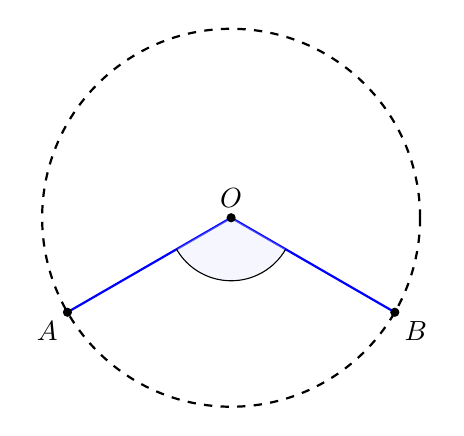
\begin{tikzpicture}[scale=1.2]
    \coordinate (O) at (0,0);
    \coordinate (A) at (210:2);
    \coordinate (B) at (330:2);
    \draw[thick, dashed] (O) circle (2);
    \draw[thick, blue] (A) -- (O) -- (B);
    \pic [draw, fill=blue!10, fill opacity=0.35, angle radius=8mm,
        pic text options={text=black}] {angle = A--O--B};
    \filldraw (O) circle (1.2pt) node[above] {$O$};
    \filldraw (A) circle (1.2pt) node[below left] {$A$};
    \filldraw (B) circle (1.2pt) node[below right] {$B$};
\end{tikzpicture}
\end{center}

\begin{definition}[\vocab{Lanko dydis ir jo žymėjimas}]
Lanko laipsninis matas lygus jį atitinkančio centrinio kampo dydžiui. Lankas žymimas lenktu ženklu virš jo galų. Pavyzdžiui, jei $\angle AOB=120^\circ$, tai lanką $\wideparen{AB}$ žymime taip:
\[ \wideparen{AB} = 120^\circ \]
\end{definition}

\begin{center}
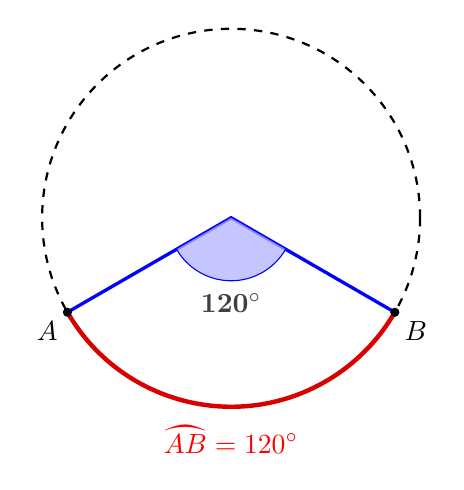
\begin{tikzpicture}[scale=1.2]
    \coordinate (O) at (0,0);
    \coordinate (A) at (210:2);
    \coordinate (B) at (330:2);
    \draw[thick, dashed] (O) circle (2);
    \draw[ultra thick, red!85!black] (210:2) arc (210:330:2);
    \draw[very thick, blue] (A) -- (O) -- (B);
    \pic [draw=blue, fill=blue!30, fill opacity=0.75, "$\mathbf{120^\circ}$", angle radius=8mm,
        angle eccentricity=1.35, pic text options={text=black, font=\bfseries}] {angle = A--O--B};
    \filldraw (A) circle (1.2pt) node[below left] {$A$};
    \filldraw (B) circle (1.2pt) node[below right] {$B$};
    \node[red, below, yshift=-1mm] at (270:2) {$\wideparen{AB} = 120^\circ$};
\end{tikzpicture}
\end{center}

\begin{definition}
\vocab{Įbrėžtinis kampas} yra kampas, kurio viršūnė yra ant apskritimo, o kampo kraštinės yra apskritimo stygos.
\end{definition}

\begin{center}
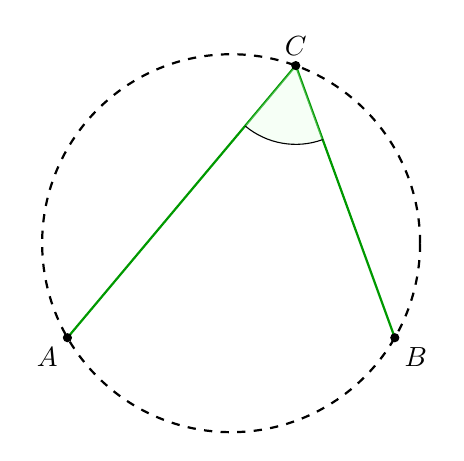
\begin{tikzpicture}[scale=1.2]
    \coordinate (A) at (210:2);
    \coordinate (B) at (330:2);
    \coordinate (C) at (70:2);
    \draw[thick, dashed] (0,0) circle (2);
    \draw[thick, green!60!black] (A) -- (C) -- (B);
    \pic [draw, fill=green!10, fill opacity=0.35, angle radius=10mm,
        pic text options={text=black}] {angle = A--C--B};
    \filldraw (A) circle (1.2pt) node[below left] {$A$};
    \filldraw (B) circle (1.2pt) node[below right] {$B$};
    \filldraw (C) circle (1.2pt) node[above] {$C$};
\end{tikzpicture}
\end{center}
\vspace{0.3cm}

\subsection{Centrinio ir įbrėžtinio kampų teorema}
\begin{theorem}[Centrinio ir įbrėžtinio kampų teorema]
Tegu $O$ yra apskritimo centras, o $A$, $B$ ir $C$ – apskritimo taškai. Jei centrinis kampas $\angle AOB$ ir įbrėžtinis kampas $\angle ACB$ remiasi į tą patį lanką $\wideparen{AB}$, tai
\[
\angle AOB=2\angle ACB.
\]
\end{theorem}
\begin{proof}
Įrodymui nubrėšime pagalbinį skersmenį per įbrėžtinio kampo viršūnę. Tuomet pritaikysime lygiašonio trikampio kampų savybę ir trikampio priekampio teoremą.

\textbf{1 žingsnis} Pažymėkime apskritimo centrą $O$ ir ant apskritimo esančius taškus $A$, $B$ bei $C$. Nubrėžkime spindulius $OA$, $OB$ ir stygas $CA$, $CB$. Taip gauname centrinį kampą $\angle AOB$ ir įbrėžtinį kampą $\angle ACB$, kurie remiasi į tą patį lanką $\wideparen{AB}$.

\begin{center}
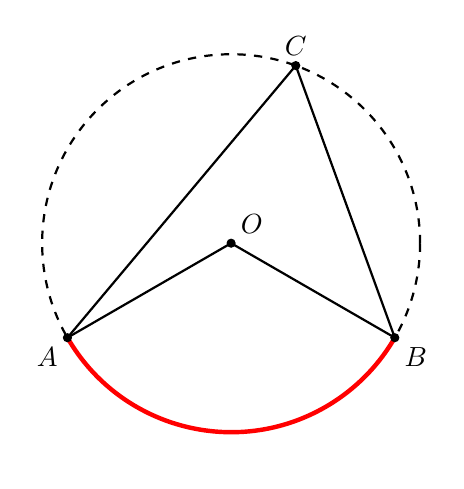
\begin{tikzpicture}[scale=1.2]
    \coordinate (O) at (0,0);
    \coordinate (A) at (210:2);
    \coordinate (B) at (330:2);
    \coordinate (C) at (70:2);
    \draw[thick, dashed] (O) circle (2);
    \draw[ultra thick, red] (210:2) arc (210:330:2);
    \draw[thick] (A) -- (O) -- (B);
    \draw[thick] (A) -- (C) -- (B);
    \foreach \p in {O,A,B,C} {\filldraw (\p) circle (1.2pt);}
    \node[above right] at (O) {$O$};
    \node[below left] at (A) {$A$};
    \node[below right] at (B) {$B$};
    \node[above] at (C) {$C$};
\end{tikzpicture}
\end{center}

\textbf{2 žingsnis} Per taškus $C$ ir $O$ nubrėžkime skersmenį $CD$. Jis padalija kampą $\angle ACB$ į du kampus. Pažymėkime juos $\alpha$ ir $\beta$.

\begin{center}
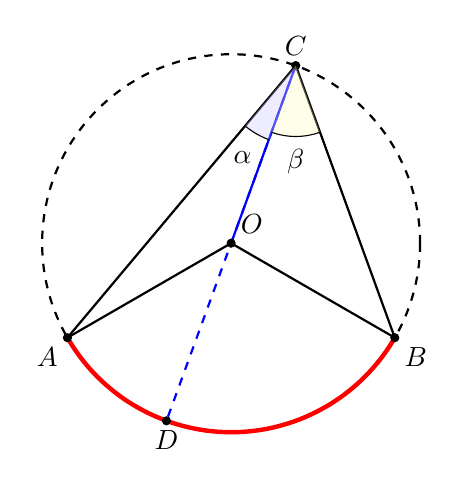
\begin{tikzpicture}[scale=1.2]
    \coordinate (O) at (0,0);
    \coordinate (A) at (210:2);
    \coordinate (B) at (330:2);
    \coordinate (C) at (70:2);
    \coordinate (D) at (250:2);
    \draw[thick, dashed] (O) circle (2);
    \draw[ultra thick, red] (210:2) arc (210:330:2);
    \draw[thick] (A) -- (O) -- (B);
    \draw[thick] (A) -- (C) -- (B);
    \draw[thick, dashed, blue] (C) -- (D);
    \draw[thick, blue] (O) -- (C);
    \foreach \p in {O,A,B,C,D} {\filldraw (\p) circle (1.2pt);}
    \pic [draw, fill=blue!20, fill opacity=0.35, "$\alpha$", angle radius=10mm, angle eccentricity=1.35,
        pic text options={text=black,text opacity=1}] {angle = A--C--D};
    \pic [draw, fill=yellow!25, fill opacity=0.35, "$\beta$", angle radius=9mm, angle eccentricity=1.35,
        pic text options={text=black,text opacity=1}] {angle = D--C--B};
    \node[above right] at (O) {$O$};
    \node[below left] at (A) {$A$};
    \node[below right] at (B) {$B$};
    \node[above] at (C) {$C$};
    \node[below] at (D) {$D$};
\end{tikzpicture}
\end{center}

\textbf{3 žingsnis} Atkarpos $OA$, $OB$ ir $OC$ yra apskritimo spinduliai, todėl $OA=OC$ ir $OB=OC$. Taigi trikampiai $\triangle AOC$ ir $\triangle BOC$ yra lygiašoniai. Kadangi $C$, $O$ ir $D$ yra vienoje tiesėje, jų kampai prie pagrindų lygūs atitinkamai $\alpha$ ir $\beta$:
\[
\angle OAC=\angle OCA=\alpha,\qquad \angle OBC=\angle OCB=\beta.
\]

\begin{center}
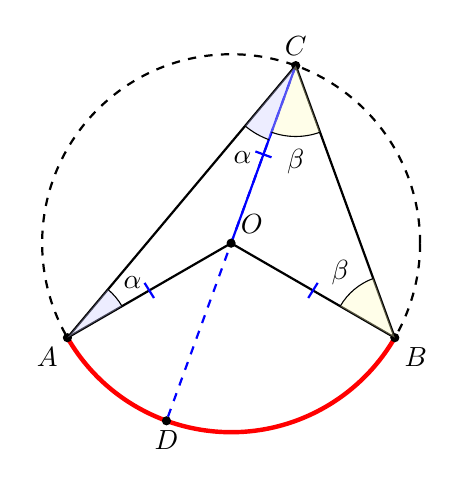
\begin{tikzpicture}[scale=1.2]
    \coordinate (O) at (0,0);
    \coordinate (A) at (210:2);
    \coordinate (B) at (330:2);
    \coordinate (C) at (70:2);
    \coordinate (D) at (250:2);
    \draw[thick, dashed] (O) circle (2);
    \draw[ultra thick, red] (210:2) arc (210:330:2);
    \draw[thick] (A) -- (O) -- (B);
    \draw[thick] (A) -- (C) -- (B);
    \draw[thick, dashed, blue] (C) -- (D);
    \draw[thick, blue] (O) -- (C);
    \foreach \p in {O,A,B,C,D} {\filldraw (\p) circle (1.2pt);}
    \draw[thick, blue] ($(O)!0.5!(A) + (-0.05, 0.08)$) -- ($(O)!0.5!(A) + (0.05, -0.08)$);
    \draw[thick, blue] ($(O)!0.5!(C) + (-0.085, 0.031)$) -- ($(O)!0.5!(C) + (0.085, -0.031)$);
    \draw[thick, blue] ($(O)!0.5!(B) + (0.05, 0.08)$) -- ($(O)!0.5!(B) + (-0.05, -0.08)$);
    \pic [draw, fill=blue!20, fill opacity=0.35, "$\alpha$", angle radius=10mm, angle eccentricity=1.35,
        pic text options={text=black,text opacity=1}] {angle = A--C--D};
    \pic [draw, fill=blue!20, fill opacity=0.35, "$\alpha$", angle radius=8mm, angle eccentricity=1.35,
        pic text options={text=black,text opacity=1}] {angle = O--A--C};
    \pic [draw, fill=yellow!25, fill opacity=0.35, "$\beta$", angle radius=9mm, angle eccentricity=1.35,
        pic text options={text=black,text opacity=1}] {angle = D--C--B};
    \pic [draw, fill=yellow!25, fill opacity=0.35, "$\beta$", angle radius=8mm, angle eccentricity=1.35,
        pic text options={text=black,text opacity=1}] {angle = C--B--O};
    \node[above right] at (O) {$O$};
    \node[below left] at (A) {$A$};
    \node[below right] at (B) {$B$};
    \node[above] at (C) {$C$};
    \node[below] at (D) {$D$};
\end{tikzpicture}
\end{center}

\textbf{4 žingsnis. Pirmasis priekampis.} Trikampio $\triangle AOC$ priekampis $\angle AOD$ lygus dviejų su juo negretimų vidaus kampų sumai, todėl: 
\[
\angle AOD=\alpha+\alpha=2\alpha.
\]

\begin{center}
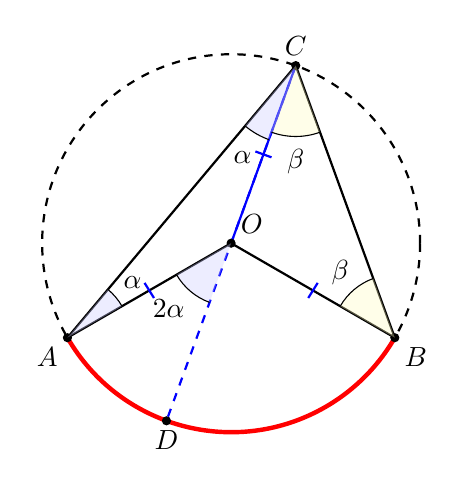
\begin{tikzpicture}[scale=1.2]
    \coordinate (O) at (0,0);
    \coordinate (A) at (210:2);
    \coordinate (B) at (330:2);
    \coordinate (C) at (70:2);
    \coordinate (D) at (250:2);
    \draw[thick, dashed] (O) circle (2);
    \draw[ultra thick, red] (210:2) arc (210:330:2);
    \draw[thick] (A) -- (O) -- (B);
    \draw[thick] (A) -- (C) -- (B);
    \draw[thick, dashed, blue] (C) -- (D);
    \draw[thick, blue] (O) -- (C);
    \foreach \p in {O,A,B,C,D} {\filldraw (\p) circle (1.2pt);}
    \draw[thick, blue] ($(O)!0.5!(A) + (-0.05, 0.08)$) -- ($(O)!0.5!(A) + (0.05, -0.08)$);
    \draw[thick, blue] ($(O)!0.5!(C) + (-0.085, 0.031)$) -- ($(O)!0.5!(C) + (0.085, -0.031)$);
    \draw[thick, blue] ($(O)!0.5!(B) + (0.05, 0.08)$) -- ($(O)!0.5!(B) + (-0.05, -0.08)$);
    \pic [draw, fill=blue!20, fill opacity=0.35, "$\alpha$", angle radius=10mm, angle eccentricity=1.35,
        pic text options={text=black,text opacity=1}] {angle = A--C--D};
    \pic [draw, fill=blue!20, fill opacity=0.35, "$\alpha$", angle radius=8mm, angle eccentricity=1.35,
        pic text options={text=black,text opacity=1}] {angle = O--A--C};
    \pic [draw, fill=yellow!25, fill opacity=0.35, "$\beta$", angle radius=9mm, angle eccentricity=1.35,
        pic text options={text=black,text opacity=1}] {angle = D--C--B};
    \pic [draw, fill=yellow!25, fill opacity=0.35, "$\beta$", angle radius=8mm, angle eccentricity=1.35,
        pic text options={text=black,text opacity=1}] {angle = C--B--O};
    \pic [draw, fill=blue!20, fill opacity=0.35, "$2\alpha$", angle radius=8mm, angle eccentricity=1.35,
        pic text options={text=black,text opacity=1, xshift=-1mm}] {angle = A--O--D};
    \node[above right] at (O) {$O$};
    \node[below left] at (A) {$A$};
    \node[below right] at (B) {$B$};
    \node[above] at (C) {$C$};
    \node[below] at (D) {$D$};
\end{tikzpicture}
\end{center}

\textbf{5 žingsnis. Antrasis priekampis.} Analogiškai trikampio $\triangle BOC$ priekampis $\angle BOD$ lygus kampų $\angle OBC$ ir $\angle OCB$ sumai, todėl: 
\[
\angle BOD=\beta+\beta=2\beta.
\]

\begin{center}
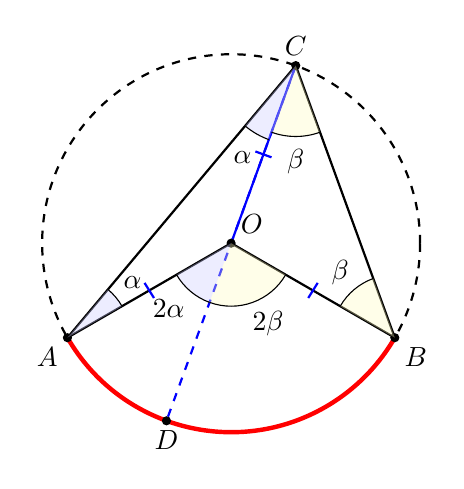
\begin{tikzpicture}[scale=1.2]
    \coordinate (O) at (0,0);
    \coordinate (A) at (210:2);
    \coordinate (B) at (330:2);
    \coordinate (C) at (70:2);
    \coordinate (D) at (250:2);
    \draw[thick, dashed] (O) circle (2);
    \draw[ultra thick, red] (210:2) arc (210:330:2);
    \draw[thick] (A) -- (O) -- (B);
    \draw[thick] (A) -- (C) -- (B);
    \draw[thick, dashed, blue] (C) -- (D);
    \draw[thick, blue] (O) -- (C);
    \foreach \p in {O,A,B,C,D} {\filldraw (\p) circle (1.2pt);}
    \draw[thick, blue] ($(O)!0.5!(A) + (-0.05, 0.08)$) -- ($(O)!0.5!(A) + (0.05, -0.08)$);
    \draw[thick, blue] ($(O)!0.5!(C) + (-0.085, 0.031)$) -- ($(O)!0.5!(C) + (0.085, -0.031)$);
    \draw[thick, blue] ($(O)!0.5!(B) + (0.05, 0.08)$) -- ($(O)!0.5!(B) + (-0.05, -0.08)$);
    \pic [draw, fill=blue!20, fill opacity=0.35, "$\alpha$", angle radius=10mm, angle eccentricity=1.35,
        pic text options={text=black,text opacity=1}] {angle = A--C--D};
    \pic [draw, fill=blue!20, fill opacity=0.35, "$\alpha$", angle radius=8mm, angle eccentricity=1.35,
        pic text options={text=black,text opacity=1}] {angle = O--A--C};
    \pic [draw, fill=yellow!25, fill opacity=0.35, "$\beta$", angle radius=9mm, angle eccentricity=1.35,
        pic text options={text=black,text opacity=1}] {angle = D--C--B};
    \pic [draw, fill=yellow!25, fill opacity=0.35, "$\beta$", angle radius=8mm, angle eccentricity=1.35,
        pic text options={text=black,text opacity=1}] {angle = C--B--O};
    \pic [draw, fill=blue!20, fill opacity=0.35, "$2\alpha$", angle radius=8mm, angle eccentricity=1.35,
        pic text options={text=black,text opacity=1, xshift=-1mm}] {angle = A--O--D};
    \pic [draw, fill=yellow!25, fill opacity=0.35, "$2\beta$", angle radius=8mm, angle eccentricity=1.35,
        pic text options={text=black,text opacity=1, xshift=1mm}] {angle = D--O--B};
    \node[above right] at (O) {$O$};
    \node[below left] at (A) {$A$};
    \node[below right] at (B) {$B$};
    \node[above] at (C) {$C$};
    \node[below] at (D) {$D$};
\end{tikzpicture}
\end{center}

\textbf{6 žingsnis. Išvada.} Centrinis kampas $\angle AOB$ sudarytas iš kampų $\angle AOD$ ir $\angle DOB$, o įbrėžtinis kampas $\angle ACB$ – iš kampų $\alpha$ ir $\beta$. Taigi
\[
\angle AOB=2\alpha+2\beta=2(\alpha+\beta)=2\angle ACB.
\]



\end{proof}

\subsection{Centrinio ir įbrėžtinio kampų teoremos išvados}
Iš įrodytos teoremos išplaukia dvi naudingos išvados.
\begin{corollary}[Į tą patį lanką besiremiantys kampai]
Tegu $C_1$ ir $C_2$ yra apskritimo taškai, esantys toje pačioje stygos $AB$ pusėje. Tuomet į tą patį lanką $\wideparen{AB}$ besiremiantys įbrėžtiniai kampai $AC_1B$ ir $AC_2B$ yra lygūs:
\[
\angle AC_1B=\angle AC_2B.
\]
\end{corollary}
\begin{proof}
Tegu $C_1$ ir $C_2$ yra du apskritimo taškai, iš kurių matomas tas pats lankas $\wideparen{AB}$. Pagal centrinio ir įbrėžtinio kampų teoremą:
\[
\angle AC_1B=\frac{1}{2}\angle AOB,
\qquad
\angle AC_2B=\frac{1}{2}\angle AOB.
\]
Taigi $\angle AC_1B=\angle AC_2B$, vadinasi, abu įbrėžtiniai kampai yra lygūs.
\end{proof}

\begin{center}
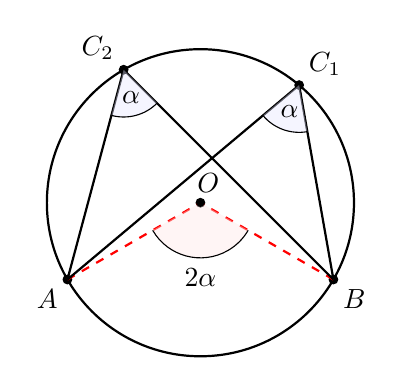
\begin{tikzpicture}[scale=1.3]
    \coordinate (O) at (0,0);
    \draw[thick] (O) circle (1.5);
    \coordinate (A) at (210:1.5);
    \coordinate (B) at (330:1.5);
    \coordinate (C1) at (50:1.5);
    \coordinate (C2) at (120:1.5);
    \foreach \p in {O,A,B,C1,C2} {\filldraw (\p) circle (1.2pt);}
    \draw[thick, dashed, red] (A) -- (O) -- (B);
    \draw[thick] (A) -- (C1) -- (B);
    \draw[thick] (A) -- (C2) -- (B);
    \pic [draw, fill=red!10, fill opacity=0.4, "$2\alpha$", angle radius=7mm, angle eccentricity=1.35,
        pic text options={text=black,text opacity=1}] {angle = A--O--B};
    \pic [draw, fill=blue!10, fill opacity=0.4, "$\alpha$", angle radius=6mm,
        pic text options={text=black,text opacity=1}] {angle = A--C1--B};
    \pic [draw, fill=blue!10, fill opacity=0.4, "$\alpha$", angle radius=6mm,
        pic text options={text=black,text opacity=1}] {angle = A--C2--B};
    \filldraw (O) circle (1pt) node[above, xshift=1mm] {$O$};
    \node[below left] at (A) {$A$};
    \node[below right] at (B) {$B$};
    \node[above right] at (C1) {$C_1$};
    \node[above left] at (C2) {$C_2$};
\end{tikzpicture}
\end{center}

\begin{corollary}[Į skersmenį besiremiantis kampas]
Tegu $AB$ yra apskritimo skersmuo, o $C$ – kitas apskritimo taškas. Tuomet į skersmenį $AB$ besiremiantis įbrėžtinis kampas $\angle ACB$ yra status:
\[
\angle ACB=90^\circ.
\]
\end{corollary}
\begin{proof}
Tegu $AB$ yra apskritimo skersmuo, o $C$ – kitas apskritimo taškas. Centrinis kampas $\angle AOB$ yra ištiestinis, todėl jo dydis $180^\circ$. Pagal centrinio ir įbrėžtinio kampų teoremą:
\[
\angle ACB=\frac{1}{2}\angle AOB=\frac{180^\circ}{2}=90^\circ.
\]
Taigi į skersmenį besiremiantis įbrėžtinis kampas yra status.
\end{proof}

\begin{center}
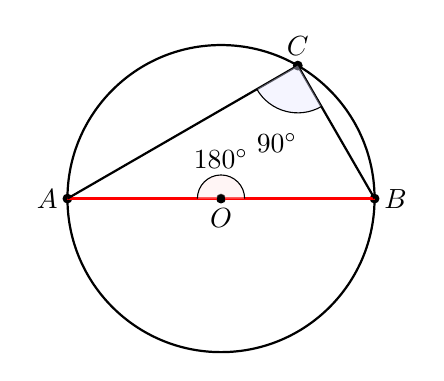
\begin{tikzpicture}[scale=1.3]
    \coordinate (O) at (0,0);
    \draw[thick] (O) circle (1.5);
    \coordinate (A) at (180:1.5);
    \coordinate (B) at (0:1.5);
    \coordinate (C) at (60:1.5);
    \foreach \p in {O,A,B,C} {\filldraw (\p) circle (1.2pt);}
    \draw[thick, red] (A) -- (B);
    \draw[thick] (A) -- (C) -- (B);
    \pic [draw, fill=red!10, fill opacity=0.4, "$180^\circ$", angle radius=3mm, angle eccentricity=1.35,
        pic text options={text=black,text opacity=1,yshift=1mm}] {angle = B--O--A};
    \pic [draw, fill=blue!10, fill opacity=0.4, "$90^\circ$", angle radius=6mm, angle eccentricity=1.7,
        pic text options={text=black,text opacity=1}] {angle = A--C--B};
    \filldraw (O) circle (1pt) node[below] {$O$};
    \node[left] at (A) {$A$};
    \node[right] at (B) {$B$};
    \node[above] at (C) {$C$};
\end{tikzpicture}
\end{center}

% ==========================================
% PAVYZDŽIAI
% ==========================================
\section{Pavyzdžiai: apskritimo savybių taikymas}

Panagrinėkime, kaip aptartos savybės padeda spręsti uždavinius.

\iffalse % Teoremos įrodymas pateiktas 2.2 poskyryje.
\begin{example}[Centrinio ir įbrėžtinio kampų ryšys]
Įrodykite, kad į tą patį lanką besiremiančio centrinio kampo dydis yra du kartus didesnis už įbrėžtinio kampo dydį.
\end{example}

\begin{proof}
Įrodymui pasitelksime lygiašonių trikampių kampų savybę ir trikampio priekampio teoremą.

\textbf{1 žingsnis.} Apskritimo centras yra $O$. Pažymėkime įbrėžtinį kampą $\angle ACB$ ir centrinį kampą $\angle AOB$. Per taškus $C$ ir $O$ nubrėžkime skersmenį $CD$. Jis padalija kampą $\angle ACB$ į dvi dalis, kurias pažymėkime $\alpha$ ir $\beta$.

\begin{center}
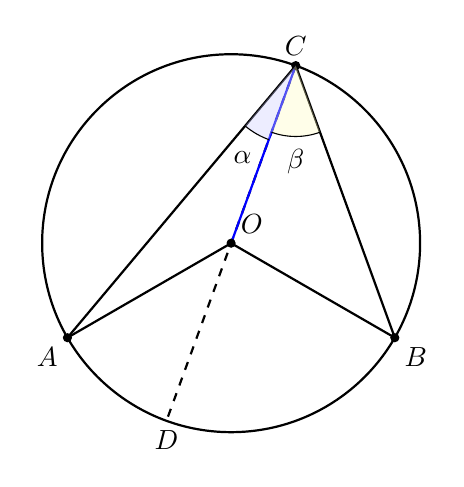
\begin{tikzpicture}[scale=1.2]
    \coordinate (O) at (0,0);
    \draw[thick] (O) circle (2);
    
    \coordinate (A) at (210:2);
    \coordinate (B) at (330:2);
    \coordinate (C) at (70:2);
    \coordinate (D) at (250:2); % skersmens pabaiga
    
    \draw[thick, dashed] (C) -- (D);
    \draw[thick] (A) -- (C) -- (B);
    \draw[thick] (A) -- (O) -- (B);
    \draw[thick, blue] (O) -- (C);
        \foreach \p in {O,A,B,C} {\filldraw (\p) circle (1.2pt);}
    
    \pic [draw, fill=blue!20, fill opacity=0.35, "$\alpha$", angle radius=10mm, angle eccentricity=1.35,
        pic text options={text=black,text opacity=1}] {angle = A--C--D};
    \pic [draw, fill=yellow!25, fill opacity=0.35, "$\beta$", angle radius=9mm, angle eccentricity=1.35,
        pic text options={text=black,text opacity=1}] {angle = D--C--B};
    
    \filldraw (O) circle (1pt) node[above right] {$O$};
    \node[below left] at (A) {$A$};
    \node[below right] at (B) {$B$};
    \node[above] at (C) {$C$};
    \node[below] at (D) {$D$};
\end{tikzpicture}
\end{center}

\textbf{2 žingsnis.} Atkarpos $OA$, $OB$ ir $OC$ yra to paties apskritimo spinduliai, todėl $OA=OC$ ir $OB=OC$. Vadinasi, trikampiai $\triangle AOC$ ir $\triangle BOC$ yra lygiašoniai. Jų kampai prie pagrindų lygūs:
\[
\angle OAC=\angle OCA=\alpha,\qquad \angle OBC=\angle OCB=\beta.
\]

\begin{center}
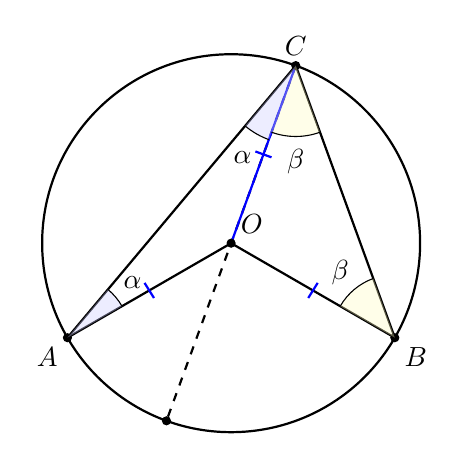
\begin{tikzpicture}[scale=1.2]
    \coordinate (O) at (0,0);
    \draw[thick] (O) circle (2);
    \coordinate (A) at (210:2); \coordinate (B) at (330:2); \coordinate (C) at (70:2); \coordinate (D) at (250:2);
    \draw[thick, dashed] (C) -- (D); \draw[thick] (A) -- (C) -- (B); \draw[thick] (A) -- (O) -- (B); \draw[thick, blue] (O) -- (C);
    \foreach \p in {O,A,B,C,D} {\filldraw (\p) circle (1.2pt);}
    
    \draw[thick, blue] ($(O)!0.5!(A) + (-0.05, 0.08)$) -- ($(O)!0.5!(A) + (0.05, -0.08)$);
    \draw[thick, blue] ($(O)!0.5!(C) + (-0.085, 0.031)$) -- ($(O)!0.5!(C) + (0.085, -0.031)$);
    \draw[thick, blue] ($(O)!0.5!(B) + (0.05, 0.08)$) -- ($(O)!0.5!(B) + (-0.05, -0.08)$);
    
    \pic [draw, fill=blue!20, fill opacity=0.35, "$\alpha$", angle radius=10mm, angle eccentricity=1.35,
        pic text options={text=black,text opacity=1}] {angle = A--C--D};
    \pic [draw, fill=blue!20, fill opacity=0.35, "$\alpha$", angle radius=8mm, angle eccentricity=1.35,
        pic text options={text=black,text opacity=1}] {angle = O--A--C};
    \pic [draw, fill=yellow!25, fill opacity=0.35, "$\beta$", angle radius=9mm, angle eccentricity=1.35,
        pic text options={text=black,text opacity=1}] {angle = D--C--B};
    \pic [draw, fill=yellow!25, fill opacity=0.35, "$\beta$", angle radius=8mm, angle eccentricity=1.35,
        pic text options={text=black,text opacity=1}] {angle = C--B--O};
    
    \filldraw (O) circle (1pt) node[above right] {$O$};
    \node[below left] at (A) {$A$}; \node[below right] at (B) {$B$}; \node[above] at (C) {$C$};
\end{tikzpicture}
\end{center}

\textbf{3 žingsnis.} Trikampyje $\triangle AOC$ kampas $\angle AOD$ yra priekampis, todėl lygus dviejų su juo negretimų vidaus kampų sumai. Taigi $\angle AOD=\alpha+\alpha=2\alpha$. Analogiškai, trikampyje $\triangle BOC$:
\[
\angle BOD=\beta+\beta=2\beta.
\]

\begin{center}
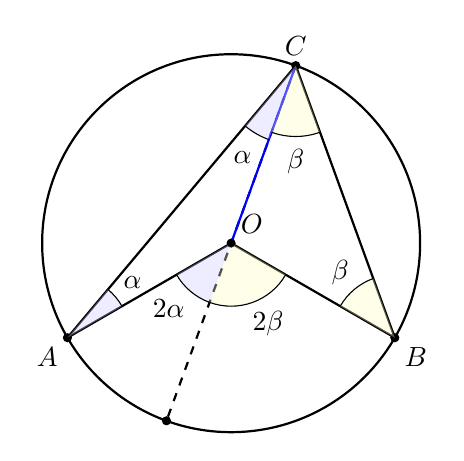
\begin{tikzpicture}[scale=1.2]
    \coordinate (O) at (0,0);
    \draw[thick] (O) circle (2);
    \coordinate (A) at (210:2); \coordinate (B) at (330:2); \coordinate (C) at (70:2); \coordinate (D) at (250:2);
    \draw[thick, dashed] (C) -- (D); \draw[thick] (A) -- (C) -- (B); \draw[thick] (A) -- (O) -- (B); \draw[thick, blue] (O) -- (C);
    \foreach \p in {O,A,B,C,D} {\filldraw (\p) circle (1.2pt);}
    
    \pic [draw, fill=blue!20, fill opacity=0.35, "$\alpha$", angle radius=10mm, angle eccentricity=1.35,
        pic text options={text=black,text opacity=1}] {angle = A--C--D};
    \pic [draw, fill=blue!20, fill opacity=0.35, "$\alpha$", angle radius=8mm, angle eccentricity=1.35,
        pic text options={text=black,text opacity=1}] {angle = O--A--C};
    \pic [draw, fill=yellow!25, fill opacity=0.35, "$\beta$", angle radius=9mm, angle eccentricity=1.35,
        pic text options={text=black,text opacity=1}] {angle = D--C--B};
    \pic [draw, fill=yellow!25, fill opacity=0.35, "$\beta$", angle radius=8mm, angle eccentricity=1.35,
        pic text options={text=black,text opacity=1}] {angle = C--B--O};

    \pic [draw, fill=blue!20, fill opacity=0.35, "$2\alpha$", angle radius=8mm, angle eccentricity=1.35,
        pic text options={text=black,text opacity=1, xshift=-1mm}] {angle = A--O--D};
    \pic [draw, fill=yellow!25, fill opacity=0.35, "$2\beta$", angle radius=8mm, angle eccentricity=1.35,
        pic text options={text=black,text opacity=1, xshift=1mm}] {angle = D--O--B};
    
    \filldraw (O) circle (1pt);
    \node[above right] at (O) {$O$};
    \node[below left] at (A) {$A$}; \node[below right] at (B) {$B$}; \node[above] at (C) {$C$};
\end{tikzpicture}
\end{center}

\textbf{4 žingsnis.} Įbrėžtinis kampas lygus $\alpha+\beta$, o centrinis kampas lygus $2\alpha+2\beta$. Todėl
\[
\angle AOB=2(\alpha+\beta)=2\angle ACB.
\]
Taigi teiginys įrodytas. \hfill $\square$
\end{proof}
\fi

\vspace{0.5cm}

% IŠVADOS

Iš įrodyto centrinio ir įbrėžtinio kampų ryšio išplaukia dar dvi naudingos išvados.

\begin{example}[Kampas tarp besikertančių stygų]
Taškai $A, B, C, D$ išsidėstę ant apskritimo. Stygos $AC$ ir $BD$ susikerta taške $E$. Duota, kad $\angle BAC = \alpha$, o $\angle ACD = \beta$. Įrodykite, kad kampas tarp dviejų besikertančių stygų $\angle BEC = \alpha + \beta$.
\end{example}

\begin{center}
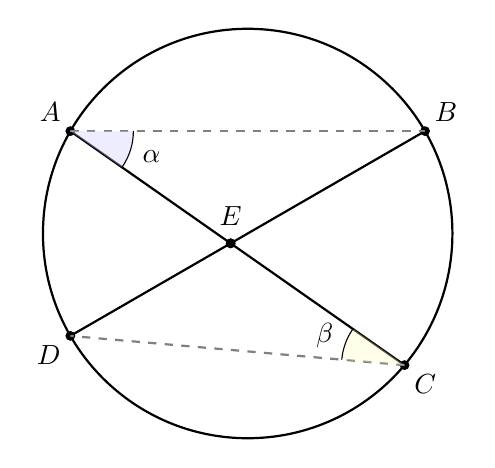
\begin{tikzpicture}[scale=1.3]
    \draw[thick] (0,0) circle (2);
    \coordinate (A) at (150:2);
    \coordinate (B) at (30:2);
    \coordinate (C) at (320:2);
    \coordinate (D) at (210:2);
    \coordinate (E) at (intersection of A--C and B--D);
    \foreach \p in {A,B,C,D,E} {\filldraw (\p) circle (1.2pt);}

    \draw[thick] (A) -- (E) -- (C);
    \draw[thick] (B) -- (E) -- (D);
    \draw[thick, gray, dashed] (A) -- (B);
    \draw[thick, gray, dashed] (C) -- (D);

    \filldraw (E) circle (1.2pt);
    \pic[draw, fill=blue!20, fill opacity=0.35, "$\alpha$", angle radius=8mm, angle eccentricity=1.35,
        pic text options={text=black,text opacity=1}] {angle = C--A--B};
    \pic[draw, fill=yellow!25, fill opacity=0.35, "$\beta$", angle radius=8mm, angle eccentricity=1.35,
        pic text options={text=black,text opacity=1}] {angle = A--C--D};
    \node[above left] at (A) {$A$};
    \node[above right] at (B) {$B$};
    \node[below right] at (C) {$C$};
    \node[below left] at (D) {$D$};
    \node[above, yshift=1mm] at (E) {$E$};
\end{tikzpicture}
\end{center}

\begin{proof}
Sąlygoje kampo $\angle BEC$ dydis nenurodytas. Jį rasime dviem žingsniais: pirmiausia pasinaudosime įbrėžtinių kampų savybe, tada – trikampio priekampio teorema.

\textbf{1 žingsnis.} Kampai $\angle ACD$ ir $\angle ABD$ remiasi į tą patį lanką $\wideparen{AD}$, todėl jie lygūs:
\[
\angle ABD = \angle ACD = \mathbf{\beta}.
\]

\begin{center}
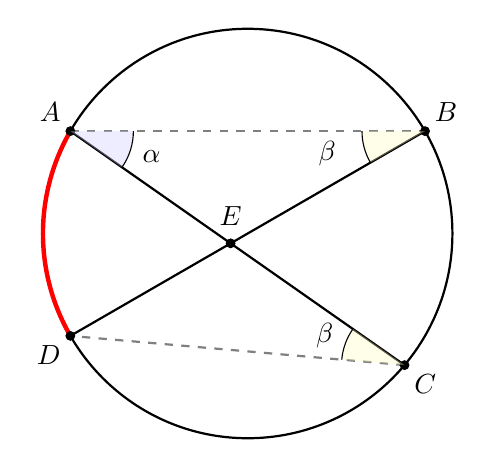
\begin{tikzpicture}[scale=1.3]
    \coordinate (O) at (0,0);
    \draw[thick] (O) circle (2);
    
    \coordinate (A) at (150:2);
    \coordinate (B) at (30:2);
    \coordinate (C) at (320:2);
    \coordinate (D) at (210:2);
    \coordinate (E) at (intersection of A--C and B--D);
    
    \draw[ultra thick, red] (150:2) arc (150:210:2); % lankas AD
    
    \draw[thick] (A) -- (C);
    \draw[thick] (B) -- (D);
    \draw[thick, gray, dashed] (C) -- (D);
    \draw[thick, gray, dashed] (A) -- (B);
    \foreach \p in {A,B,C,D,E} {\filldraw (\p) circle (1.2pt);}
    
    \pic [draw, fill=blue!20, fill opacity=0.35, "$\alpha$", angle radius=8mm, angle eccentricity=1.35,
        pic text options={text=black,text opacity=1}] {angle = C--A--B};
    \pic [draw, fill=yellow!25, fill opacity=0.35, "$\beta$", angle radius=8mm, angle eccentricity=1.35,
        pic text options={text=black,text opacity=1}] {angle = A--C--D};
    \pic [draw, fill=yellow!25, fill opacity=0.35, "$\beta$", angle radius=8mm, angle eccentricity=1.35,
        pic text options={text=black,text opacity=1, xshift=-2mm}] {angle = A--B--D};
    
    \node[above left] at (A) {$A$};
    \node[above right] at (B) {$B$};
    \node[below right] at (C) {$C$};
    \node[below left] at (D) {$D$};
    \node[above, yshift=1mm] at (E) {$E$};
\end{tikzpicture}
\end{center}

\textbf{2 žingsnis.} Nagrinėkime trikampį $\triangle ABE$. Kadangi taškas $E$ priklauso atkarpoms $AC$ ir $BD$, turime $\angle BAE=\angle BAC=\alpha$ ir $\angle ABE=\angle ABD=\beta$. Kampas $\angle BEC$ yra trikampio $\triangle ABE$ priekampis ties viršūne $E$, todėl
\[
\angle BEC = \angle BAE + \angle ABE = \alpha + \beta.
\]
Vadinasi, ieškomo kampo dydis yra $\alpha+\beta$. Teiginys įrodytas. \hfill $\square$
\end{proof}

\newpage
\begin{example}[Pusiaukraštinė stačiajame trikampyje]
Trikampis $\triangle ABC$ yra statusis, $\angle C=90^\circ$. Taškas $M$ yra įžambinės $AB$ vidurys, todėl $AM=MB$. Įrodykite, kad $CM=AM=MB$.
\end{example}

\begin{center}
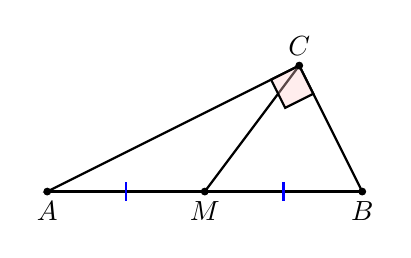
\begin{tikzpicture}[scale=1]
    \coordinate (A) at (-2,0); \coordinate (B) at (2,0);
    \coordinate (C) at (1.2,1.6); \coordinate (M) at (0,0);
    \draw[thick] (A) -- (C) -- (B) -- cycle;
    \draw[thick] (C) -- (M); \draw[thick] (A) -- (M) -- (B);
    \draw[thick, blue] ($(A)!0.5!(M)+(0,0.12)$) -- ($(A)!0.5!(M)+(0,-0.12)$);
    \draw[thick, blue] ($(M)!0.5!(B)+(0,0.12)$) -- ($(M)!0.5!(B)+(0,-0.12)$);
    \coordinate (CdirA) at ($(C)!4mm!(A)$);
    \coordinate (CdirB) at ($(C)!4mm!(B)$);
    \coordinate (Crect) at ($(CdirA) + (CdirB) - (C)$);
    \draw[thick, fill=red!20, fill opacity=0.35] (CdirA) -- (Crect) -- (CdirB) -- (C) -- cycle;
    \filldraw (A) circle (1.2pt); \filldraw (B) circle (1.2pt);
    \filldraw (C) circle (1.2pt); \filldraw (M) circle (1.2pt);
    \node[below] at (A) {$A$}; \node[below] at (B) {$B$};
    \node[above] at (C) {$C$}; \node[below] at (M) {$M$};
\end{tikzpicture}
\end{center}

\begin{proof}
Šį uždavinį jau nagrinėjome ankstesniame handoute. Dabar jį išspręsime pasinaudodami apskritimo savybėmis.

\textbf{1 žingsnis.} Kadangi $\angle C=90^\circ$, trikampį $ABC$ galima įbrėžti į apskritimą, kurio skersmuo yra $AB$. Kadangi $M$ yra šio skersmens vidurio taškas, jis yra apskritimo centras.

\begin{center}
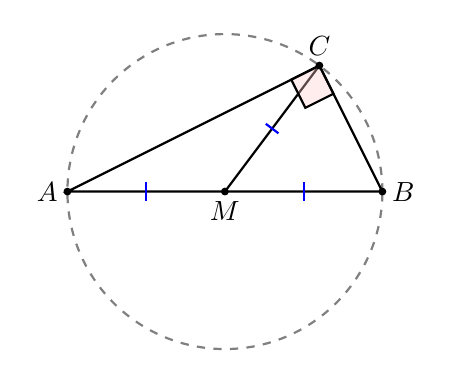
\begin{tikzpicture}[scale=1]
    \coordinate (M) at (0,0);
    \coordinate (A) at (-2,0);
    \coordinate (B) at (2,0);
    \coordinate (C) at (1.2,1.6);
    \draw[thick, dashed, gray] (M) circle (2);
    \draw[thick] (A)--(C)--(B)--cycle;
    \draw[thick] (M)--(C);
    \draw[thick, blue] ($(A)!0.5!(M)+(0,0.12)$)--($(A)!0.5!(M)+(0,-0.12)$);
    \draw[thick, blue] ($(M)!0.5!(B)+(0,0.12)$)--($(M)!0.5!(B)+(0,-0.12)$);
    \draw[thick, blue] ($(M)!0.5!(C)+(-0.08,0.06)$)--($(M)!0.5!(C)+(0.08,-0.06)$);
    \coordinate (CdirA) at ($(C)!4mm!(A)$);
    \coordinate (CdirB) at ($(C)!4mm!(B)$);
    \coordinate (Crect) at ($(CdirA)+(CdirB)-(C)$);
    \draw[thick, fill=red!20, fill opacity=0.35] (CdirA)--(Crect)--(CdirB)--(C)--cycle;
    \filldraw (M) circle (1.2pt); \filldraw (A) circle (1.2pt);
    \filldraw (B) circle (1.2pt); \filldraw (C) circle (1.2pt);
    \node[below] at (M) {$M$}; \node[left] at (A) {$A$};
    \node[right] at (B) {$B$}; \node[above] at (C) {$C$};
\end{tikzpicture}
\end{center}

\textbf{2 žingsnis.} Atkarpos $MA$, $MB$ ir $MC$ yra to paties apskritimo spinduliai, todėl
\[
MA=MB=MC.
\]

\begin{center}
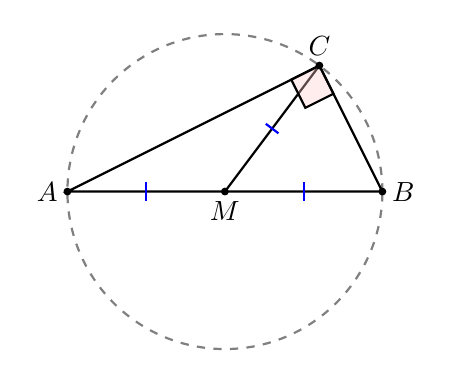
\begin{tikzpicture}[scale=1]
    \coordinate (M) at (0,0);
    \coordinate (A) at (-2,0);
    \coordinate (B) at (2,0);
    \coordinate (C) at (1.2,1.6);
    \draw[thick, dashed, gray] (M) circle (2);
    \draw[thick] (A)--(C)--(B)--cycle;
    \draw[thick] (M)--(C);
    \draw[thick, blue] ($(A)!0.5!(M)+(0,0.12)$)--($(A)!0.5!(M)+(0,-0.12)$);
    \draw[thick, blue] ($(M)!0.5!(B)+(0,0.12)$)--($(M)!0.5!(B)+(0,-0.12)$);
    \draw[thick, blue] ($(M)!0.5!(C)+(-0.08,0.06)$)--($(M)!0.5!(C)+(0.08,-0.06)$);
    \coordinate (CdirA) at ($(C)!4mm!(A)$);
    \coordinate (CdirB) at ($(C)!4mm!(B)$);
    \coordinate (Crect) at ($(CdirA)+(CdirB)-(C)$);
    \draw[thick, fill=red!20, fill opacity=0.35] (CdirA)--(Crect)--(CdirB)--(C)--cycle;
    \filldraw (M) circle (1.2pt); \filldraw (A) circle (1.2pt);
    \filldraw (B) circle (1.2pt); \filldraw (C) circle (1.2pt);
    \node[below] at (M) {$M$}; \node[left] at (A) {$A$};
    \node[right] at (B) {$B$}; \node[above] at (C) {$C$};
\end{tikzpicture}
\end{center}

\textbf{3 žingsnis.} Kadangi $M$ yra atkarpos $AB$ vidurio taškas, $AM=MB$. Be to, $MA$, $MB$ ir $MC$ yra to paties apskritimo spinduliai, todėl
\[
CM=AM=MB.
\]
Taigi pusiaukraštinė $CM$ lygi pusei įžambinės. Teiginys įrodytas. \hfill $\square$
\end{proof}
\vspace{0.5cm}

% ==========================================
% UŽDAVINIAI
% ==========================================
\newpage
\begin{example}[Apskritime įbrėžta trapecija]
Apskritime nubrėžtos dvi lygiagrečios stygos $AB \parallel CD$. Įrodykite, kad gautas keturkampis $ABCD$ yra lygiašonė trapecija, t. y. $AD=BC$.
\end{example}

\begin{center}
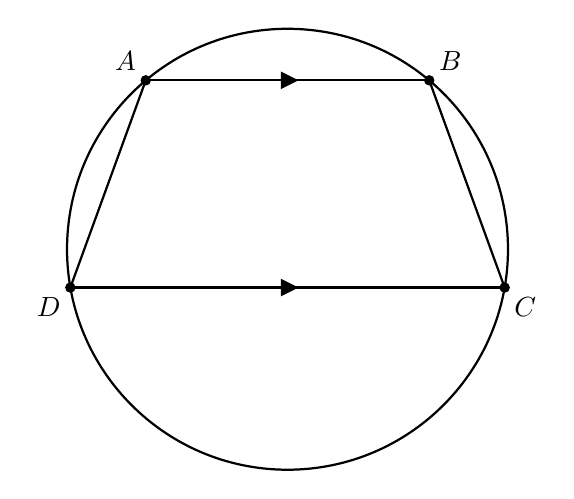
\begin{tikzpicture}[scale=1.4]
    \coordinate (O) at (0,0);
    \draw[thick] (O) circle (2);
    
    \coordinate (A) at (130:2);
    \coordinate (B) at (50:2);
    \coordinate (C) at (350:2);
    \coordinate (D) at (190:2);
    
    \draw[thick] (A) -- (B);
    \draw[thick] (C) -- (D);
    \draw[thick] (A) -- (D);
    \draw[thick] (B) -- (C);
    
    % Lygiagretumo rodyklės
    \fill[black] ($(A)!0.5!(B)+(0.10,0)$) --
        ($(A)!0.5!(B)+(-0.06,0.08)$) --
        ($(A)!0.5!(B)+(-0.06,-0.08)$) -- cycle;
    \fill[black] ($(D)!0.5!(C)+(0.10,0)$) --
        ($(D)!0.5!(C)+(-0.06,0.08)$) --
        ($(D)!0.5!(C)+(-0.06,-0.08)$) -- cycle;
    
    \foreach \p in {A,B,C,D} {\filldraw (\p) circle (1.2pt);}
    
    \node[above left] at (A) {$A$};
    \node[above right] at (B) {$B$};
    \node[below right] at (C) {$C$};
    \node[below left] at (D) {$D$};
\end{tikzpicture}
\end{center}

\begin{proof}
Nubrėžkime įstrižainę $AC$ ir susiekime lygiagrečių tiesių sudaromus kampus su atitinkamais apskritimo lankais.

\textbf{1 žingsnis.} Kadangi $AB\parallel CD$, vidaus priešiniai kampai yra lygūs:
\[
\angle BAC = \angle ACD = \mathbf{\alpha}.
\]

\begin{center}
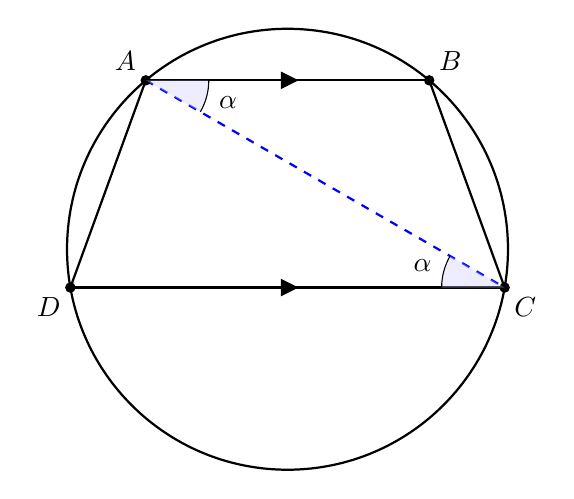
\begin{tikzpicture}[scale=1.4]
    \coordinate (O) at (0,0);
    \draw[thick] (O) circle (2);
    
    \coordinate (A) at (130:2);
    \coordinate (B) at (50:2);
    \coordinate (C) at (350:2);
    \coordinate (D) at (190:2);
    
    \draw[thick] (A) -- (B);
    \draw[thick] (C) -- (D);
    \draw[thick] (A) -- (D);
    \draw[thick] (B) -- (C);
    \draw[thick, dashed, blue] (A) -- (C);
    \fill[black] ($(A)!0.5!(B)+(0.10,0)$) --
        ($(A)!0.5!(B)+(-0.06,0.08)$) --
        ($(A)!0.5!(B)+(-0.06,-0.08)$) -- cycle;
    \fill[black] ($(D)!0.5!(C)+(0.10,0)$) --
        ($(D)!0.5!(C)+(-0.06,0.08)$) --
        ($(D)!0.5!(C)+(-0.06,-0.08)$) -- cycle;
    
    \foreach \p in {A,B,C,D} {\filldraw (\p) circle (1.2pt);}
    
    \pic [draw, fill=blue!20, fill opacity=0.35, "$\alpha$", angle radius=8mm, angle eccentricity=1.35,
        pic text options={text=black,text opacity=1}] {angle = C--A--B};
    \pic [draw, fill=blue!20, fill opacity=0.35, "$\alpha$", angle radius=8mm, angle eccentricity=1.35,
        pic text options={text=black,text opacity=1}] {angle = A--C--D};
    
    \node[above left] at (A) {$A$}; \node[above right] at (B) {$B$};
    \node[below right] at (C) {$C$}; \node[below left] at (D) {$D$};
\end{tikzpicture}
\end{center}

\textbf{2 žingsnis.} Įbrėžtinis kampas $\angle BAC=\alpha$ remiasi į lanką $\wideparen{BC}$, todėl $\wideparen{BC}=2\alpha$. Taip pat kampas $\angle ACD=\alpha$ remiasi į lanką $\wideparen{AD}$, vadinasi, $\wideparen{AD}=2\alpha$. Taigi lankai $\wideparen{AD}$ ir $\wideparen{BC}$ yra lygūs.

\begin{center}
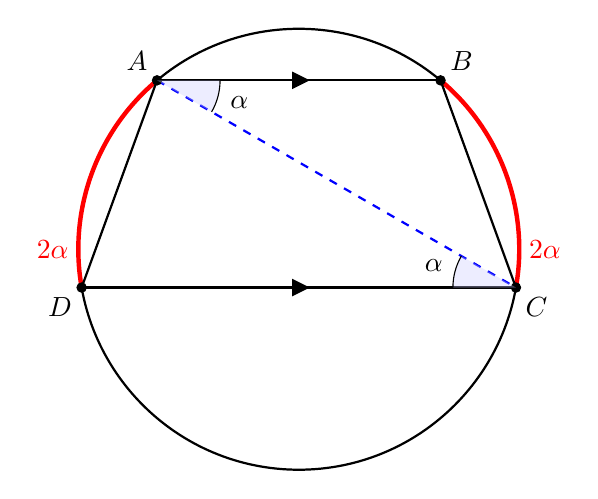
\begin{tikzpicture}[scale=1.4]
    \coordinate (O) at (0,0);
    \draw[thick] (O) circle (2);
    
    \coordinate (A) at (130:2); \coordinate (B) at (50:2);
    \coordinate (C) at (350:2); \coordinate (D) at (190:2);
    
    \draw[ultra thick, red] (50:2) arc (50:-10:2); % lankas BC
    \draw[ultra thick, red] (130:2) arc (130:190:2); % lankas AD
    
    \draw[thick] (A) -- (B); \draw[thick] (C) -- (D);
    \draw[thick] (A) -- (D); \draw[thick] (B) -- (C);
    \draw[thick, dashed, blue] (A) -- (C);
    \fill[black] ($(A)!0.5!(B)+(0.10,0)$) --
        ($(A)!0.5!(B)+(-0.06,0.08)$) --
        ($(A)!0.5!(B)+(-0.06,-0.08)$) -- cycle;
    \fill[black] ($(D)!0.5!(C)+(0.10,0)$) --
        ($(D)!0.5!(C)+(-0.06,0.08)$) --
        ($(D)!0.5!(C)+(-0.06,-0.08)$) -- cycle;
    
    \foreach \p in {A,B,C,D} {\filldraw (\p) circle (1.2pt);}
    
    \pic [draw, fill=blue!20, fill opacity=0.35, "$\alpha$", angle radius=8mm, angle eccentricity=1.35,
        pic text options={text=black,text opacity=1}] {angle = C--A--B};
    \pic [draw, fill=blue!20, fill opacity=0.35, "$\alpha$", angle radius=8mm, angle eccentricity=1.35,
        pic text options={text=black,text opacity=1}] {angle = A--C--D};
        
    \node[red, right] at (0:2) {$2\alpha$};
    \node[red, left] at (180:2) {$2\alpha$};
    
    \node[above left] at (A) {$A$}; \node[above right] at (B) {$B$};
    \node[below right] at (C) {$C$}; \node[below left] at (D) {$D$};
\end{tikzpicture}
\end{center}

\textbf{3 žingsnis.} Sujunkime apskritimo centrą $O$ su taškais $A$, $B$, $C$ ir $D$. Kadangi $OA=OB=OC=OD$, o lygūs lankai $\wideparen{AD}$ ir $\wideparen{BC}$ atitinka lygius centrinius kampus, tai $\angle AOD=\angle BOC$. Vadinasi, trikampiai $\triangle AOD$ ir $\triangle BOC$ lygūs pagal kraštinė–kampas–kraštinė, todėl
\[
AD = BC.
\]
Taigi $AD=BC$ ir trapecija $ABCD$ yra lygiašonė. Vadinasi, kiekviena į apskritimą įbrėžta trapecija yra lygiašonė. \hfill $\square$
\end{proof}
\newpage
\section{Uždaviniai savarankiškam sprendimui (13 uždavinių)}
\begin{enumerate}
    \renewcommand{\labelenumi}{\textbf{\theenumi.}}
    
    \item Apskritime nubrėžtas centrinis kampas $\angle AOB=130^\circ$. Raskite įbrėžtinio kampo $\angle ACB$ dydį, jei taškas $C$ yra didesniajame lanke $\wideparen{AB}$.
    \item Apskritimo styga padalija apskritimą į du lankus. Į vieną iš jų besiremiantis įbrėžtinis kampas lygus $70^\circ$. Raskite į tą patį lanką besiremiančio centrinio kampo dydį.
    \item Trikampis $\triangle ABC$ įbrėžtas į apskritimą. Žinoma, kad $\angle A = 50^\circ$, o $\angle B = 60^\circ$. Raskite visų trijų atitinkamų apskritimo lankų, į kuriuos remiasi šie kampai, dydžius (laipsniais).
    \item Taškai $A, B, C, D$ paeiliui išsidėstę ant apskritimo. Įrodykite, kad $\angle CAD=\angle CBD$ ir $\angle BCA=\angle BDA$.
    \item Taškai $A, B, C, D$ išsidėstę ant apskritimo, stygos $AC$ ir $BD$ susikerta taške $P$. Duota, kad $\angle BDC = 25^\circ$, o $\angle ACD = 45^\circ$. Apskaičiuokite kampą $\angle BPC$.
    \item Apskritime nubrėžtos stygos $AB$ ir $CD$ susikerta taške $K$. Lankų $\wideparen{AC}$ ir $\wideparen{BD}$ dydžiai yra atitinkamai $40^\circ$ ir $80^\circ$. Įrodykite, kad $\angle AKC$ lygus šių lankų dydžių sumos pusei, t. y. $60^\circ$.
    \item Atkarpa $AB$ yra apskritimo skersmuo. Ant apskritimo pažymėtas taškas $C$. Iš taško $C$ nuleista aukštinė $CH$ į skersmenį $AB$. Žinoma, kad $\angle A = 35^\circ$. Raskite kampą $\angle BCH$.
    \item Trikampyje $\triangle ABC$ kampai yra $\angle A=60^\circ$, $\angle B=70^\circ$ ir $\angle C=50^\circ$. Nubrėžtos aukštinės $AD$ ir $BE$ susikerta taške $H$.
    \begin{itemize}
        \item[a)] Įrodykite, kad keturkampis $CEHD$ yra įbrėžtinis. Nustatykite jį einančio apskritimo skersmenį.
        \item[b)] Įrodykite, kad keturkampis $ABDE$ taip pat yra įbrėžtinis.
    \end{itemize}
    \textit{Šis uždavinys susieja šiame handoute aptartas savybes su kita tema.}
    \item Stačiojo trikampio $\triangle ABC$ ($\angle C=90^\circ$) įžambinės vidurio taškas yra $M$. Trikampio aukštinė $CH$ nubrėžta į įžambinę. Įrodykite, kad $\angle MCH=\angle A-\angle B$, kai $\angle A>\angle B$.
    \item Trikampis $\triangle ABC$ įbrėžtas į apskritimą. Pusiaukampinė $AD$ kerta priešingą kraštines $BC$ taške $D$, o patį apskritimą kerta taške $M$. Įrodykite, kad taškas $M$ yra lanko $\wideparen{BC}$ vidurio taškas.
    \item Nagrinėkime smailųjį trikampį $ABC$. Aukštinės $BE$ ir $CD$ atitinkamai kerta kraštines $AC$ ir $AB$. Įrodykite, kad $\angle ADE=\angle ABC$.
    \item Apskritime nubrėžtos dvi lygiagrečios stygos $AB\parallel CD$. Įrodykite, kad tarp jų esantys lankai $\wideparen{AC}$ ir $\wideparen{BD}$ yra lygūs. Pasinaudokite įbrėžtinių kampų ir lygiagrečių tiesių savybėmis.
    \item Smailusis trikampis $\triangle ABC$ įbrėžtas į apskritimą. Taškas $M$ yra lanko $\wideparen{AB}$ vidurys, o taškas $N$ – lanko $\wideparen{AC}$ vidurys. Styga $MN$ kerta kraštines $AB$ ir $AC$ atitinkamai taškuose $X$ ir $Y$. Įrodykite, kad trikampis $\triangle AXY$ yra lygiašonis, t. y. $AX=AY$.
\end{enumerate}
\end{document}